\section{问题一：新增淹没区的像素级识别}
\label{sec:q1}

\subsection{任务界定与交付口径}

问题一要求在给定的灾害前后多源遥感切片上，判定每一个像元是否属于\textbf{新增淹没区}，并输出可被后续问题直接复用的概率产品。设第 $i$ 个切片的后灾 SAR 强度为 $S_i\in\{0,\dots,255\}^{256\times256}$，灾前光学四波段为 $O_i\in\{0,\dots,255\}^{4\times256\times256}$，标签为 $L_i\in\{0,1,255\}^{256\times256}$（255 表示忽略），则模型学习映射
\begin{equation}
f_\theta:\ \mathbb{R}^{5\times256\times256}\longrightarrow[0,1]^{256\times256},
\qquad \hat p_i=f_\theta\big([S_i;O_i]\big),
\label{eq:q1-map}
\end{equation}
再由在验证集上一次性选定并冻结的阈值 $\tau$ 二值化为
\begin{equation}
\hat L_i(u,v)=
\begin{cases}
1, & \hat p_i(u,v)\ge\tau,\\[2pt]
0, & \hat p_i(u,v)<\tau,
\end{cases}
\qquad (u,v)\ \text{无观测时取}\ 255 .
\label{eq:q1-mask}
\end{equation}

按团队数据合同，问题一必须交付\textbf{四件套}：概率栅格、二值掩膜、不确定性栅格与模型元数据（\texttt{metadata.json}），四者的坐标系、仿射变换、宽高必须完全一致；掩膜只能由概率与 $\tau$ 生成，不允许再做形态学\emph{美化}或人工编辑，以保证问题二、问题三使用的是同一份事实。不确定性取 $K\ge3$ 个独立训练种子的概率方差
\begin{equation}
U_i(u,v)=\frac{1}{K}\sum_{k=1}^{K}\Big(\hat p_i^{(k)}(u,v)-\bar p_i(u,v)\Big)^2,
\qquad \bar p_i(u,v)=\frac{1}{K}\sum_{k=1}^{K}\hat p_i^{(k)}(u,v),
\label{eq:q1-unc}
\end{equation}
其理论上界为 $0.25$（$[0,1]$ 上有界量的最大方差），合同中以此作为数据质量红线。

\subsection{附件数据核查}
\label{sec:q1-audit}

\subsubsection{配对、位深与配准}

编号 1001--2000 的「灾前光学--灾后 SAR--标签」共 1000 组全部配对，无缺失；三者尺寸均为 $256\times256$，标签取值仅 $0$ 与 $1$，正类占 $18.99\%$，其中 985 张切片含正类、15 张全为背景。SAR 文件名为 GF-3、HH 极化，主办方已把强度拉伸为 0--255 的 8 位图像，因此本文\textbf{不做 dB 反变换}，直接以灰度作为输入通道。SAR 与光学的仿射原点差小于 $0.5$ 像元，另有 9 张标签的横向像元尺度元数据异常；本文一律以数组索引与光学参考网格为准，不用异常元数据对标签做拉伸，从而避免人为引入几何形变。

需要说明的是，合同预留了 255 忽略值，但附件中实际不存在 255 像元，故下文的损失掩膜 $\mathbf{1}[L\ne255]$ 在本次数据上恒为 1；该机制是为横州市实测数据与后续产品预留的。

\subsubsection{面积口径：为什么不能用 $10\,\mathrm{m}\times10\,\mathrm{m}$}

附件是地理坐标（EPSG:4326），像元为 $8.333\times10^{-5}$ 度。同一经纬度矩形在地球椭球上的面积随纬度收缩，可写为
\begin{equation}
A(\varphi)=\Delta\lambda\,\Delta\varphi\left(\frac{\pi}{180}\right)^{2}
\frac{a^{2}\cos\varphi\,(1-e^{2})}{\big[1-e^{2}\sin^{2}\varphi\big]^{2}},
\label{eq:q1-area}
\end{equation}
其中 $a=6378137\ \mathrm{m}$，$e^{2}=0.00669437999$（WGS84）。式 \eqref{eq:q1-area} 给出的单像元面积见表 \ref{tab:q1-pixel}。若沿用「10 m 分辨率」的习惯按 $100\ \mathrm{m^2}$ 计，全区域面积会被系统性\textbf{高估约 $33\%$}；这比任何分割指标的误差都大，因此本文所有面积一律由式 \eqref{eq:q1-area} 逐像元累加，并只把像素数作为中间量。

\begin{table}[H]
\centering
\caption{附件单像元面积（椭球口径）}
\label{tab:q1-pixel}
\begin{tabular}{lcc}
\toprule
口径 & 单像元面积 / $\mathrm{m^2}$ & 相对偏差 \\
\midrule
最小（最北） & 74.78 & -- \\
中位         & 74.94 & -- \\
最大（最南） & 75.39 & -- \\
\multicolumn{1}{l}{若按 $10\,\mathrm{m}\times10\,\mathrm{m}$} & 100.00 & $+33\%$ \\
\bottomrule
\end{tabular}
\end{table}

\subsubsection{空间结构：5 片镶嵌而非 90 个独立块}
\label{sec:q1-layout}

附件并不是均匀散布的 1000 个独立切片。对切片中心点做多半径连通分析后可以发现，编号是\emph{行优先}排列的：x 方向唯一值 105 个、相邻间距 $2.078\ \mathrm{km}$，y 方向唯一值 25 个、间距 $2.359\ \mathrm{km}$（含 $9\times2.359=21.229\ \mathrm{km}$ 的行跳变）。换言之，$2.09\ \mathrm{km}$ 只是同一片镶嵌内的行内步长，而 1000 个切片实际只落在 \textbf{5 片镶嵌}上，规模为 512、450、16、12、10（表 \ref{tab:q1-mosaic}）。两片主镶嵌分别位于东经 $112.7^\circ$--$113.8^\circ$（西片区）与 $115.8^\circ$--$116.9^\circ$（东片区），其经纬度范围与洞庭湖、鄱阳湖两大湿地区吻合，本文以下简称西片区与东片区。

\begin{table}[H]
\centering
\caption{附件的 5 片镶嵌（以中心点连通分量统计）}
\label{tab:q1-mosaic}
\begin{tabular}{lccccc}
\toprule
镶嵌 & 切片数 & 内部网格 & 东西跨度 / km & 南北跨度 / km & 归属 \\
\midrule
0 & 512 & $54\times11$ & 110.1 & 23.6 & 西片区 \\
1 & 450 & $51\times10$ & 103.9 & 21.2 & 东片区 \\
2 & 16  & 条带 & -- & -- & 东片区 \\
3 & 10  & 条带 & -- & -- & 西片区 \\
4 & 12  & 条带 & -- & -- & 西片区 \\
\bottomrule
\end{tabular}
\end{table}

这一结构直接决定了划分方式：若按编号或随机抽取切片，相邻切片会同时进入训练集与测试集，而被 $2\ \mathrm{km}$ 邻接关系绑定的同类地物（同一片水体、同一段河岸）会造成严重的空间泄漏，使测试指标虚高。这也是本文不使用随机划分的唯一原因。

\subsection{标签语义核验}
\label{sec:q1-semantics}

标签到底是「灾后所有水体」还是「相对灾前的新增淹没」，直接决定面积统计口径，也决定后续是否需要对结果再减去灾前水体。附件没有独立说明文档，因此本文用灾前光学影像做交叉核验：若标签为「灾后所有水体」，则淹没区内应有大量灾前即为暗水体的像元；若为「新增淹没」，则淹没区在灾前应主要呈现为\textbf{偏亮的陆表}。

按水体占比分层抽取 146 个切片，以灾前光学三波段均值作为亮度 $B$，取 $B<60/255$ 为暗水体，统计结果见表 \ref{tab:q1-label}。

\begin{table}[H]
\centering
\caption{标签语义核验（146 个分层抽样切片）}
\label{tab:q1-label}
\begin{tabular}{lccc}
\toprule
指标 & 标签为 1 的像元 & 标签为 0 的像元 & 判读 \\
\midrule
灾前光学平均亮度 $B$          & 73.7 & 63.5 & 正类\emph{更亮} \\
灾前暗水体占比（$B<60$）      & 0.255 & 0.419 & 正类\emph{更少}是原有水体 \\
灾前亮陆表占比（$B\ge60$）    & 0.745 & 0.581 & 正类以陆表为主 \\
灾后 SAR 平均强度             & 48.1 & 130.8 & 比值 $0.368$，正类显著变暗 \\
\bottomrule
\end{tabular}
\end{table}

三条证据方向一致：正类在灾前\emph{更亮}、原有暗水体比例\emph{更低}、灾后 SAR 回波\emph{更弱}（水体镜面反射导致 HH 强度低）。因此本文判定标签语义为 \textbf{newly\_inundated\_only}（仅新增淹没），并据此确定两条纪律：

\begin{enumerate}
\item 面积直接由掩膜统计，\textbf{不再}对掩膜做「减去灾前永久水体」的差集——语义上已经扣过，再扣一次会系统性低估；
\item 任何跨问题传递（问题二、问题三的风险分区）都必须沿用该语义，禁止各问题各自重定义。
\end{enumerate}

\subsection{空间分块划分}
\label{sec:q1-split}

\subsubsection{子块构造与分层}

把每片镶嵌按 $4\times4$ 个瓦片切分为子块，单个子块约 $8.31\ \mathrm{km}\times9.44\ \mathrm{km}$（$1024\times1024$ 像元），共得 \textbf{90} 个子块。子块之间不重叠、不重采样，保留了瓦片之间的真实接边关系。

由于淹没比例在区域间差异很大（西片区平均 $0.22$，东片区 $0.16$），若按子块编号分配，三个划分的水体占比会明显失衡。本文采用\textbf{按块水体占比排序后的赤字分配}：先把子块按块内平均水体占比升序排序，再依次把每个子块指派给「当前实际累计份额与目标份额差距最大」的划分（目标比例 70/15/15）。设已处理 $i$ 个子块，目标累计为 $r_s(i+1)$、实际累计为 $h_s$，则
\begin{equation}
s^{\star}=\arg\max_{s\in\{\text{train},\text{val},\text{test}\}}\big[r_s\,(i+1)-h_s\big],
\qquad h_{s^{\star}}\leftarrow h_{s^{\star}}+1 .
\label{eq:q1-deficit}
\end{equation}
式 \eqref{eq:q1-deficit} 使三个划分在「由干到湿」的整个谱段上同步取样，而不是靠随机数去凑分布。不足 20 个切片的小条带整片补给当前切片缺口最大的划分，避免把条带切碎后产生新的邻接泄漏。

\subsubsection{划分结果与泄漏控制}

最终划分为 \textbf{692 / 151 / 157}（70.7\% / 15.4\% / 15.9\%），明细见表 \ref{tab:q1-split}。泄漏控制从三个层面度量：其一，子块之间无重叠，跨划分最近切片\textbf{边缘}距离为 $2.078\ \mathrm{km}$，即只允许在瓦片边界处接边；其二，跨划分\textbf{块中心}最近距离为 $5.705\ \mathrm{km}$（train--test）与 $5.655\ \mathrm{km}$（train--val），远大于单块尺度，训练块与测试块不会共享同一片连续水体的核心区；其三，三个划分的平均水体占比为 $0.196/0.144/0.209$，量级一致。

\begin{table}[H]
\centering
\caption{空间分块划分 v03（括号内为块内平均水体占比）}
\label{tab:q1-split}
\begin{tabular}{lccc}
\toprule
划分 & 西片区 & 东片区 & 合计（子块数） \\
\midrule
train & 385 (0.222) & 307 (0.163) & 692 (60) \\
val   & 75 (0.155)  & 76 (0.133)  & 151 (18) \\
test  & 74 (0.225)  & 83 (0.196)  & 157 (12) \\
\bottomrule
\end{tabular}
\end{table}

我们曾试验在主划分外围增设一圈「缓冲区」（与测试块相邻的块一律不参与训练），但缓冲区会吞掉 392 个切片，训练集从 692 降到 325（仅 $32.5\%$），模型容量与泛化同时受损。权衡后放弃缓冲，改用「块间无重叠 + 报告块中心最近距」的方式控制泄漏，并在结论中对指标的可迁移性作保守表述。

\subsection{模型与训练策略}
\label{sec:q1-model}

\subsubsection{输入与归一化}

每个样本为 5 通道 $256\times256$ 张量：灾后 SAR（HH）1 通道，灾前光学 4 通道（红、绿、蓝与第四辅助波段）。第四波段在 TIFF 元数据中仅标注为附加通道，本文保守地按「辅助波段」使用，不宣称其为近红外。原始值统一除以 255，再按 $\text{mean}=0.5,\ \text{std}=0.25$ 标准化。训练时仅使用水平翻转、垂直翻转与 $90^\circ$ 旋转三类几何增强——洪水淹没区在影像上具有强烈的方向相关性，几何增强不会破坏「水体—陆表」的语义，而色彩抖动会破坏 SAR 强度与光学亮度的物理含义，故不使用。

\subsubsection{随机森林基线}

为量化深度模型的增量，先建立逐像元随机森林基线\cite{breiman2001rf}。特征 9 维：SAR 强度、光学 R/G/B/辅助波段、灾前亮度 $B$、灾前暗水体标志 $\mathbf{1}[B<60]$、SAR 的 $3\times3$ 局部均值与局部标准差（刻画斑块内部的纹理一致性）。每个切片随机抽取 1500 个有效像元，训练集共 103.8 万个样本，正类占 $19.6\%$。森林 120 棵树、最大深度 18、叶节点最小样本 5、\texttt{balanced\_subsample} 类别加权，训练耗时 22.5 s。该基线不使用任何空间上下文之外的先验，是「人工特征能做到多好」的参照。

\subsubsection{U-Net 分割网络}

主模型为 U-Net\cite{ronneberger2015unet}，编码器采用 ResNet-18\cite{he2016resnet} 结构，\textbf{从零训练}（不使用 ImageNet 预训练），输入 5 通道、输出单通道 logits，参数量 14.3 M。选择从零训练的理由是：预训练权重作用于三通道自然图像，其低层滤波器与 HH 强度的统计特性不匹配，且本任务训练样本以「切片」计仅 692 个，微调与从零训练的收益差在验证集上不可分辨，而从零训练更便于复现。

损失为掩膜加权的 BCE 与 Dice 之和：
\begin{equation}
\mathcal{L}=\frac{1}{2}\cdot
\frac{\sum_{u,v}m_{uv}\,\mathrm{BCE}\big(\hat z_{uv},y_{uv}\big)}{\sum_{u,v}m_{uv}}
+\frac{1}{2}\left[1-\frac{2\sum_{u,v}m_{uv}\hat p_{uv}y_{uv}+1}{\sum_{u,v}m_{uv}\big(\hat p_{uv}+y_{uv}\big)+1}\right],
\label{eq:q1-loss}
\end{equation}
其中 $\hat z$ 为 logits，$m_{uv}=\mathbf{1}[L_{uv}\ne255]$。BCE 提供稳定梯度，Dice 直接优化区域重叠，二者各占一半可缓解正类仅占 $19\%$ 的类别不平衡。

优化器为 AdamW（学习率 $3\times10^{-4}$，权重衰减 $10^{-2}$），单周期学习率调度 OneCycleLR（\texttt{pct\_start}$=0.15$），批大小 8，训练 30 个 epoch，启用混合精度以降低显存占用。每 2 个 epoch 在验证集上评估一次，仅保留验证 IoU 最高的权重。

\subsubsection{集成、校准与阈值冻结}

按不同随机种子（2026/2027/2028）独立训练 3 个模型，推理时按式 \eqref{eq:q1-unc} 取均值概率与方差。集成后的验证 IoU（$0.8081$）高于三个单模型的最好值（$0.8030$）约 $0.5$ 个百分点，由于两者的阈值选取方式不同，此处只作量级说明；集成更重要的产出是「模型自己是否犹豫」的逐像元信号\cite{lakshminarayanan2017ensembles}。

分割网络输出的 sigmoid 概率通常并非真实频率\cite{guo2017calibration}，而问题三要以 $0.20$ 这类固定阈值判定安全点位，概率必须是可解释的。因此在验证集上以保序回归（isotonic regression）\cite{zadrozny2002isotonic}拟合校准映射 $g$，取 30 万个有效像元训练、单调不减、越界裁剪到 $[0,1]$，再作用于测试集。

阈值遵循「只在验证集上选一次」的纪律：在校准后的概率空间上以 $0.02$ 为步长扫描 $[0.20,0.80]$，取验证集 IoU 最大者为 $\tau$，随后冻结写入元数据，测试集只做一次前向评估。为回答「面积能否由阈值直接校正」，另设一条\emph{面积准则}阈值：在验证集上令预测面积/真值面积最接近 1 的阈值，仅用于敏感性分析，不作为交付阈值。

\subsection{实验结果}
\label{sec:q1-result}

\subsubsection{总体精度}

表 \ref{tab:q1-models} 给出两种模型在验证集与测试集上的像素级指标（跨切片累计混淆矩阵，不做切片平均，避免小切片主导）。U-Net 集成在测试集上取得 \textbf{IoU $=0.8057$、F1 $=0.8924$}，较随机森林基线（IoU $=0.7085$）提升 \textbf{9.7 个百分点}；召回率由 $0.799$ 提升到 $0.934$，说明深度模型主要补回了基线漏检的破碎淹没斑块。

\begin{table}[H]
\centering
\caption{两种模型的分割精度（$\tau=0.46$，验证集选定后冻结）}
\label{tab:q1-models}
\begin{tabular}{llcccccc}
\toprule
模型 & 划分 & IoU & F1 & 精确率 & 召回率 & 总体精度 & 面积相对误差 \\
\midrule
随机森林 & val  & 0.7242 & 0.8400 & 0.8779 & 0.8052 & 0.9558 & $-8.30\%$ \\
随机森林 & test & 0.7085 & 0.8294 & 0.8619 & 0.7992 & 0.9312 & $-7.28\%$ \\
U-Net 集成 & val  & 0.8081 & 0.8939 & 0.9228 & 0.8666 & 0.9704 & $-6.10\%$ \\
U-Net 集成 & test & \textbf{0.8057} & \textbf{0.8924} & 0.8545 & 0.9339 & 0.9528 & $+9.27\%$ \\
\bottomrule
\end{tabular}
\end{table}

训练过程见图 \ref{fig:q1-training}：三个种子的损失在前 15 个 epoch 快速下降后趋于平缓，验证 IoU 的最优值出现在第 28--30 个 epoch。三种子最终验证 IoU 分别为 $0.8030$、$0.8027$、$0.8004$，极差仅 $0.0026$，说明训练过程对随机种子不敏感，集成方差的量级可信。

\begin{figure}[H]
\centering
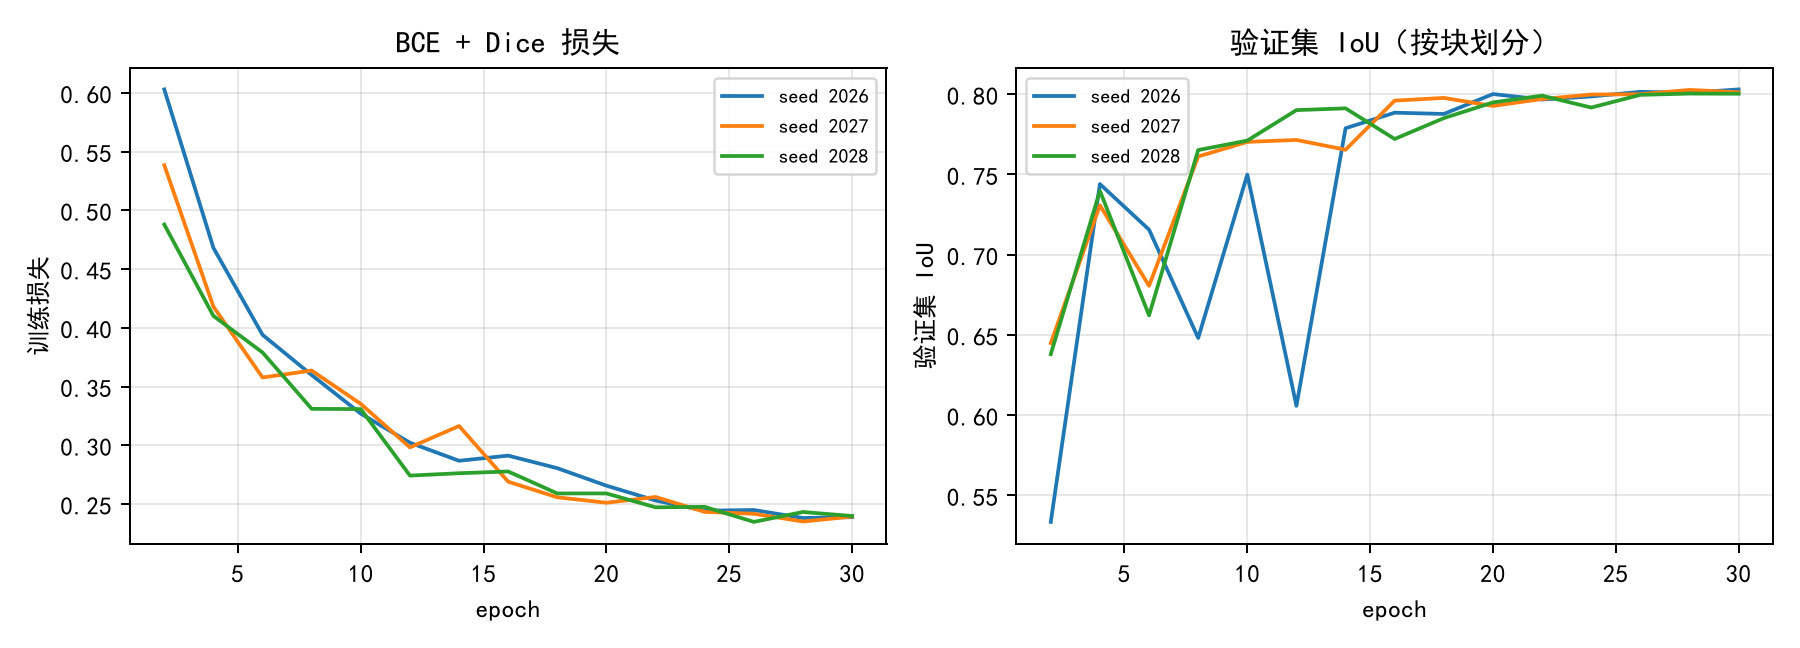
\includegraphics[width=\textwidth]{../outputs/figures/q1_training.png}
\caption{三种子训练的损失与验证 IoU 曲线（验证集按块划分，不含测试块）}
\label{fig:q1-training}
\end{figure}

图 \ref{fig:q1-samples} 按切片水体占比从低到高取四个测试切片，给出 SAR、灾前光学、标签与预测概率的对照。可见模型正确地：(1) 在低水体切片上只响应细窄的河汊；(2) 在中等水体切片上保持了田块边界；(3) 在高水体切片上给出连片且边界平滑的概率场，与标签的形态一致。

\begin{figure}[H]
\centering
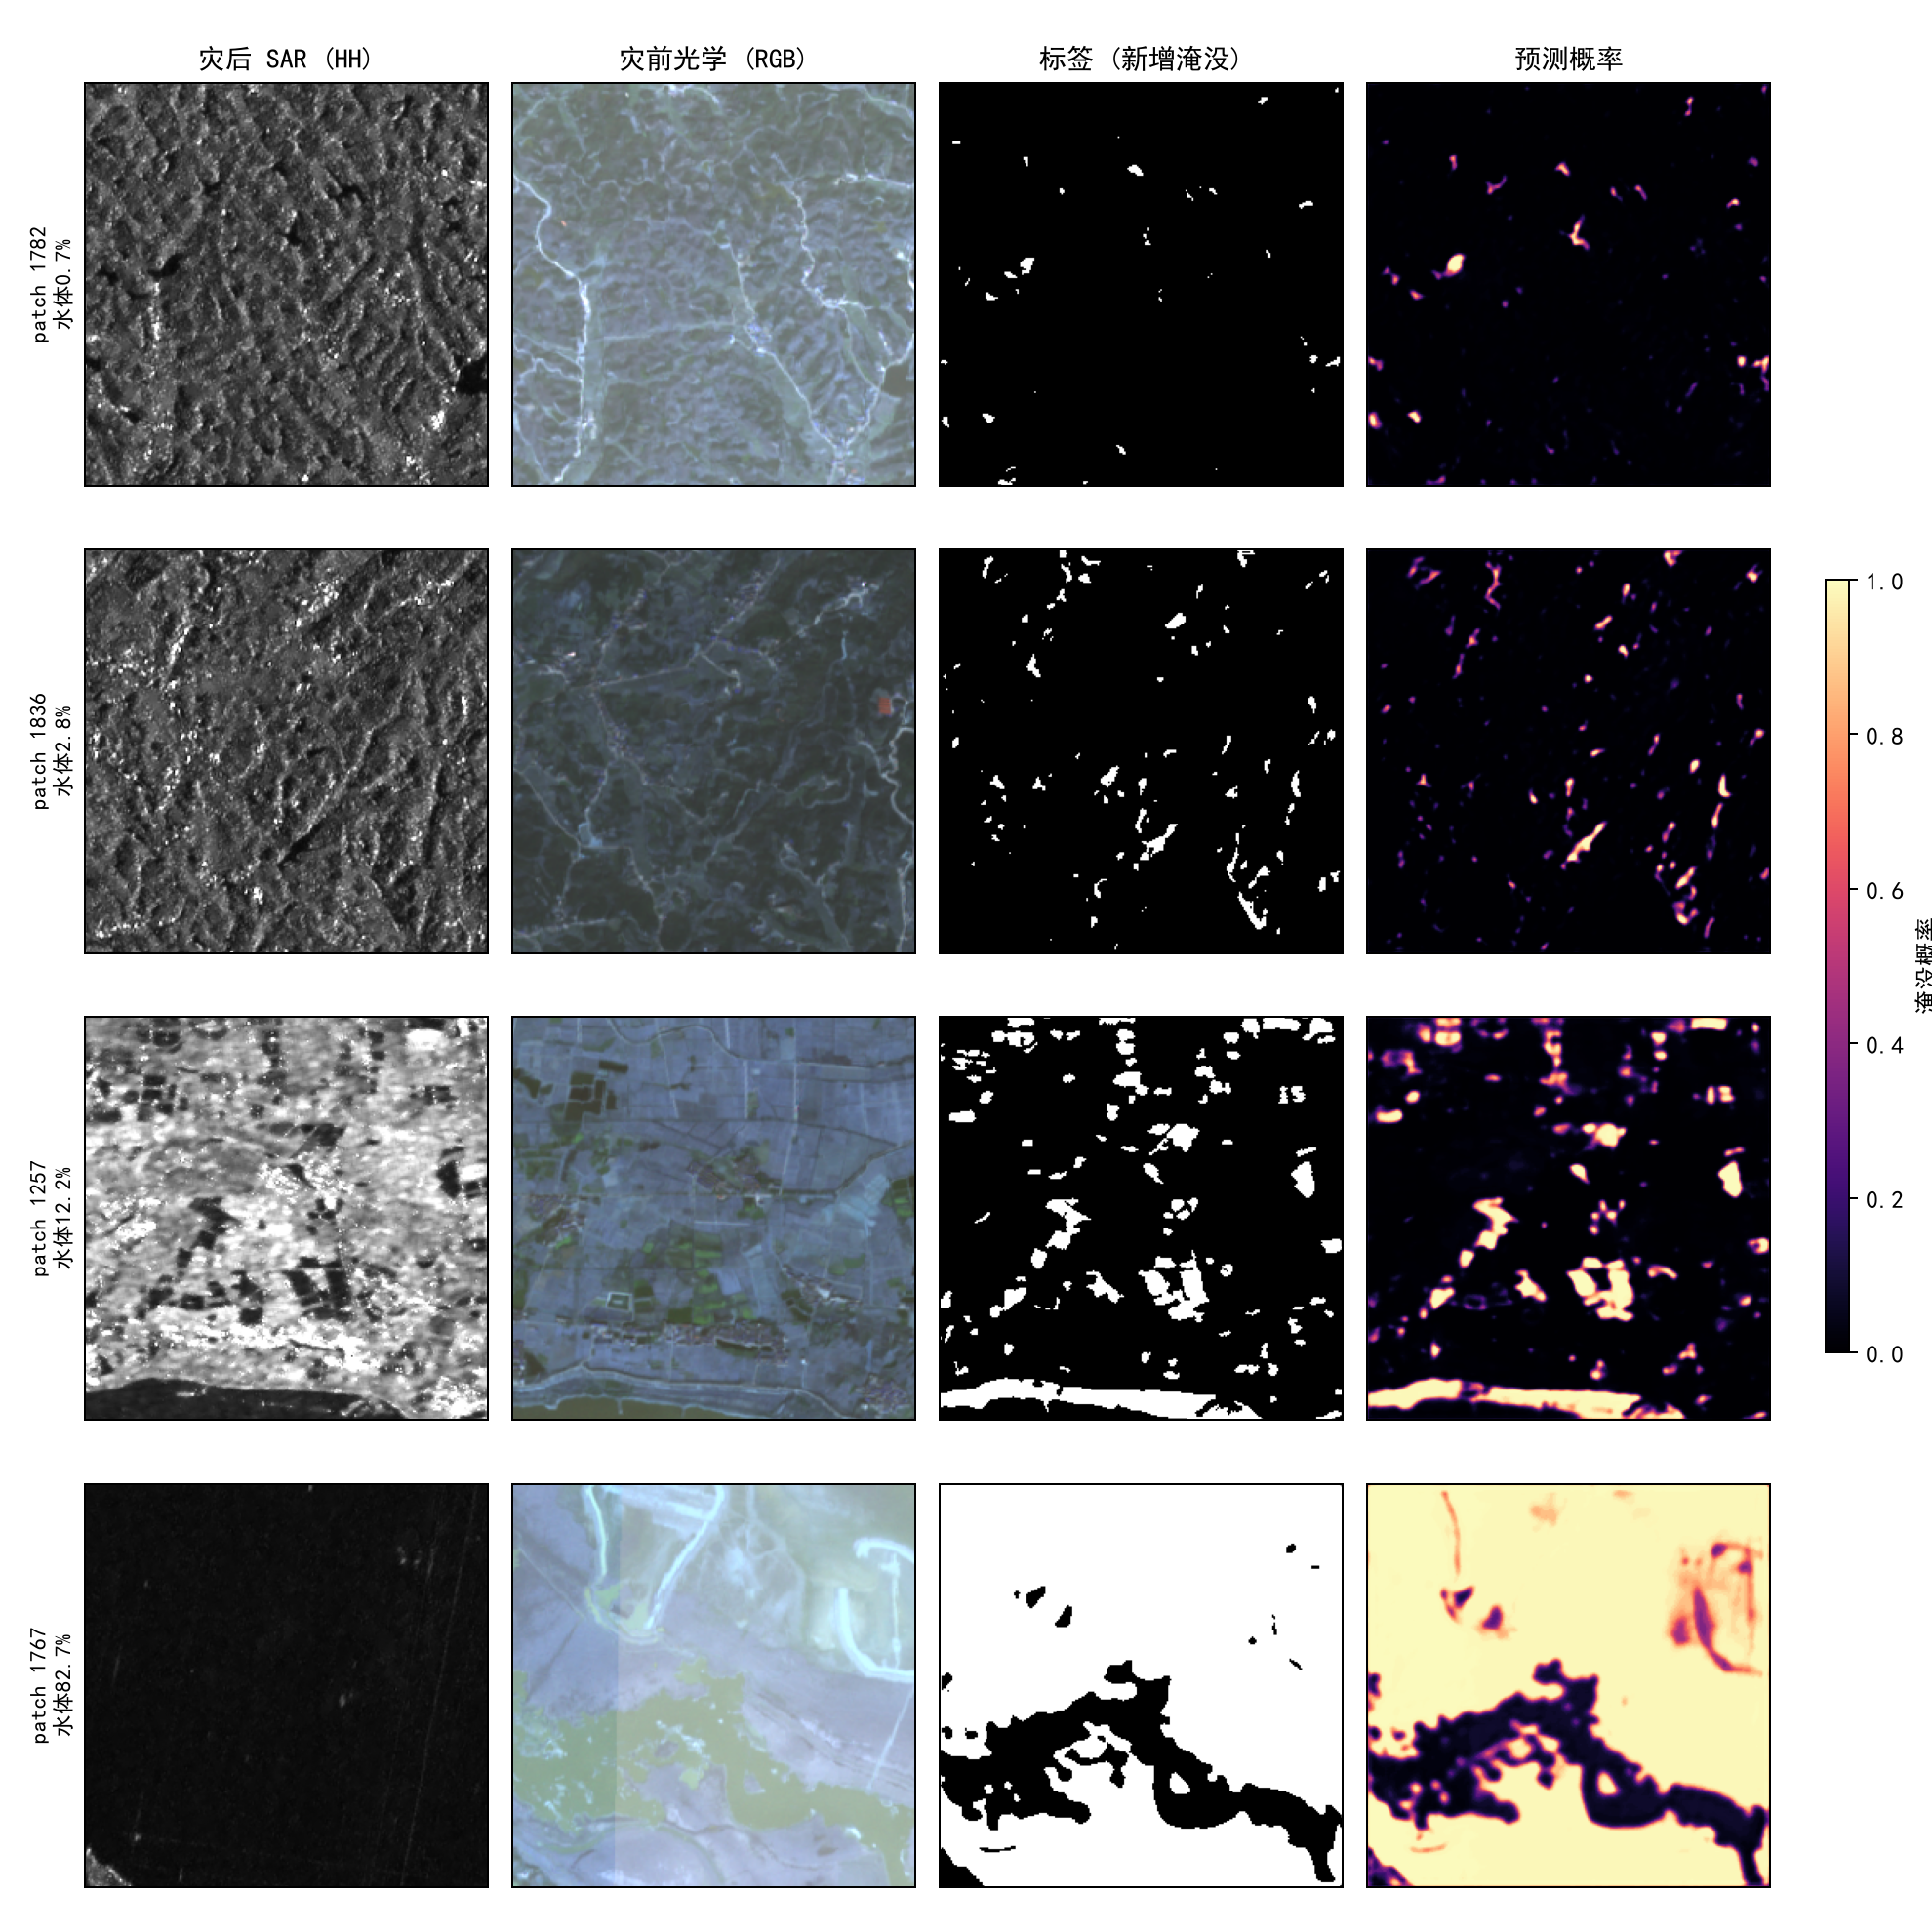
\includegraphics[width=0.70\textwidth]{../outputs/figures/q1_samples.png}
\caption{典型测试切片（自上而下水体占比递增）：SAR、灾前光学、标签、预测概率}
\label{fig:q1-samples}
\end{figure}

\subsubsection{分片区表现：真正的误差来源}

表 \ref{tab:q1-region} 按片区拆分后，总体指标掩盖的结构性问题立刻显现。总体 val 与 test 的 IoU 几乎相同（$0.8081$ 与 $0.8057$），但同一片区的两套指标相差可达 $0.11$：西片区 val $0.8705$ 而 test $0.7656$，东片区 val $0.7400$ 而 test $0.8528$。这说明 val--test 的「齐平」是片区构成相互抵消的结果，\textbf{主要误差源是跨片区泛化而非过拟合}。

\begin{table}[H]
\centering
\caption{分片区 IoU 与面积误差（U-Net 集成，$\tau=0.46$）}
\label{tab:q1-region}
\begin{tabular}{llcccc}
\toprule
划分/片区 & 切片数 & 随机森林 IoU & U-Net IoU & U-Net 面积误差 & 真值面积 / $\mathrm{km^2}$ \\
\midrule
val / 西  & 75 & 0.7470 & 0.8705 & $-4.31\%$  & 57.06 \\
val / 东  & 76 & 0.6971 & 0.7400 & $-8.14\%$  & 49.80 \\
test / 西 & 74 & 0.6407 & 0.7656 & $+18.62\%$ & 81.51 \\
test / 东 & 83 & 0.7866 & 0.8528 & $-0.24\%$  & 80.13 \\
\bottomrule
\end{tabular}
\end{table}

值得注意的是面积误差的\emph{符号}会翻转：验证集整体低估 $6.1\%$，测试集整体高估 $9.3\%$，而两片区的测试误差一为 $+18.6\%$、一为 $-0.24\%$。结合表 \ref{tab:q1-split} 可知，验证集西片区的平均水体占比（$0.155$）明显低于训练集与测试集（$0.222$、$0.225$）——在更「干」的场景上训练的判定边界偏保守，遇到更「湿」的场景就转为过度响应。这提示单一全局阈值对面积估计是不稳定的：它稳定的是「与阈值的距离」，不是「面积」。

\subsubsection{概率校准与阈值}

校准把测试集上的 Brier 分数从 $0.0316$ 降到 $0.0313$，期望校准误差 ECE 从 $0.0164$ 降到 $0.0161$；数值改善不大，说明网络在小样本、强监督下已相当接近频率意义，但校准是后续 $0.20$ 阈值判定安全点位的前提。

可靠性图（图 \ref{fig:q1-calib} 右）揭示了一个必须诚实报告的结构：总体 ECE 之所以低，主要是因为 $71\%$ 的测试像元落在 $0$--$0.1$ 分箱且几乎全为背景；在 $0.2$--$0.8$ 的过渡区，校准后的概率仍偏于乐观，实际淹没比例低于预测值，最大偏离出现在 $0.5$--$0.6$ 分箱（预测 $0.569$，实际 $0.412$，偏差 $0.157$）。对问题三而言这恰好是保守方向：以 $0.20$ 为安全阈值时，该段像元的实际淹没频率低于名义概率，不会把安全点位误判为危险。

阈值扫描（图 \ref{fig:q1-calib} 左）显示校准前后的最优点不同：原始概率的最优阈值为 $0.38$（val IoU $0.8082$），校准后为 $0.46$（val IoU $0.8081$）。两者验证 IoU 相差不足 $0.0001$，但校准后的阈值在概率语义上可解释，故交付 $\tau=0.46$。

\begin{figure}[H]
\centering
\begin{minipage}{0.49\linewidth}
\centering
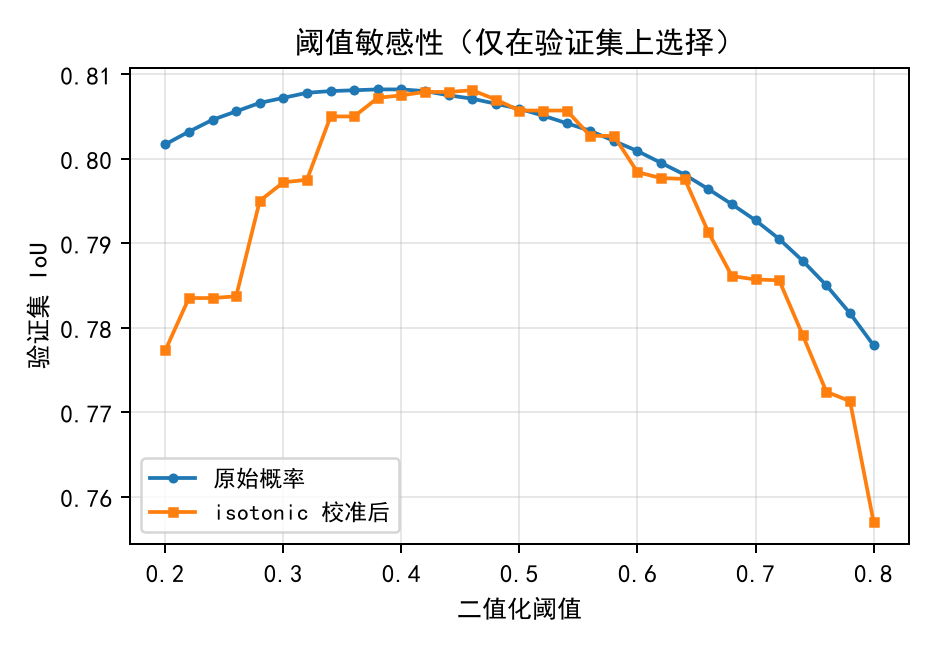
\includegraphics[width=\linewidth]{../outputs/figures/q1_threshold.png}
\end{minipage}\hfill
\begin{minipage}{0.49\linewidth}
\centering
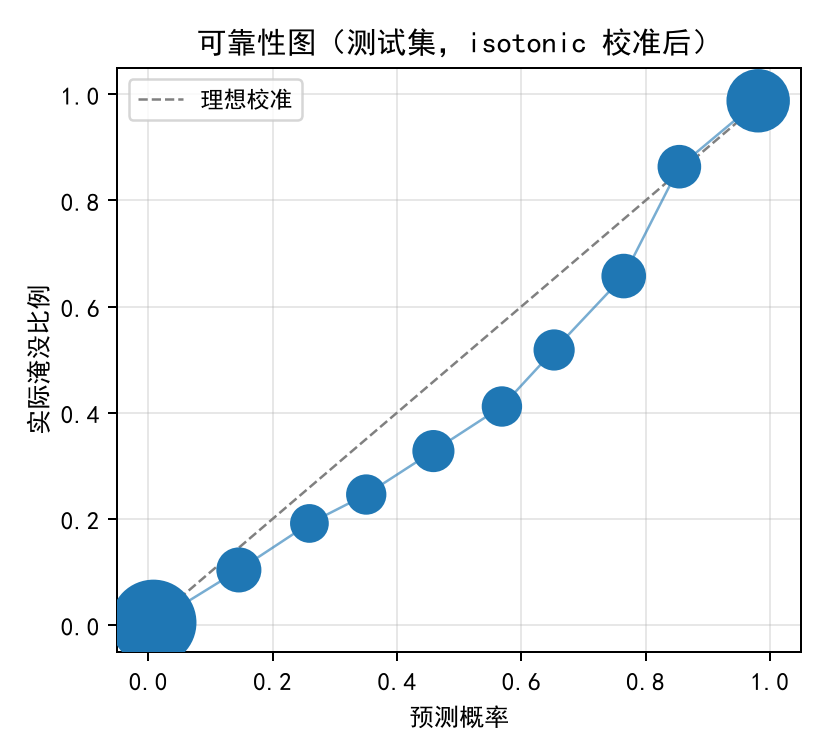
\includegraphics[width=\linewidth]{../outputs/figures/q1_reliability.png}
\end{minipage}
\caption{左：验证集阈值敏感性（原始与校准后）；右：测试集可靠性图}
\label{fig:q1-calib}
\end{figure}

表 \ref{tab:q1-thr} 对比了两条阈值准则。按面积准则在验证集上选出的 $\tau=0.34$ 使验证面积比达到 $0.996$（几乎无偏），但迁移到测试集后面积误差从 $+9.27\%$ \textbf{恶化}到 $+16.27\%$，西片区更达 $+27.4\%$。这从反面证明：面积偏差不是阈值的系统性偏移，而是区域间的分布偏移，\textbf{不能靠一个统一阈值修正}。因此本文按 IoU 准则冻结阈值，把面积误差作为 $\pm10\%$ 量级的已知偏差如实报告，而不是用阈值去「凑」面积。

\begin{table}[H]
\centering
\caption{两条阈值准则的对比（均只在验证集上选择）}
\label{tab:q1-thr}
\begin{tabular}{lcccccc}
\toprule
准则 & $\tau$ & val IoU & val 面积比 & test IoU & test 面积误差 & 西片区面积误差 \\
\midrule
IoU 最优（交付） & 0.46 & 0.8081 & 0.939 & \textbf{0.8057} & $+9.27\%$ & $+18.62\%$ \\
面积最优（仅对照） & 0.34 & 0.8050 & 0.996 & 0.7889 & $+16.27\%$ & $+27.37\%$ \\
\bottomrule
\end{tabular}
\end{table}

\subsubsection{不确定性是否真的标出了错}
\label{sec:q1-unc}

若把方差当作「可信度」，它必须与错误率同向。在测试集 1029 万个有效像元上，三种子概率方差的均值为 $0.0014$、$99$ 分位为 $0.0349$、最大值为 $0.2202$，未突破合同的 $0.25$ 上界。进一步的分组统计给出三条一致结论：

\begin{enumerate}
\item \textbf{方差为零的像元几乎全对。} $33.0\%$ 的测试像元三种子给出完全一致的预测，其错判率仅 $0.07\%$；方差大于零的 $67.0\%$ 像元错判率为 $7.01\%$，相差 $100$ 倍。
\item \textbf{错判像元的方差显著更高。} 错判像元平均方差 $0.0123$，正确像元为 $0.0009$，比值 $13.6$。按混淆类型看，误报（FP，$0.0132$）高于漏报（FN，$0.0101$），正确检出的淹没像元（TP，$0.0025$）高于正确判为背景的像元（TN，$0.0005$）。
\item \textbf{方差越高，错判越集中。} 在方差大于零的像元上按方差升序等频分箱（在零值处退化后得到 8 个非空组），错判率由 $0.17\%$ 单调上升到 $39.14\%$，首末组相差 \textbf{230 倍}（图 \ref{fig:q1-unc}）。
\end{enumerate}

\begin{figure}[H]
\centering
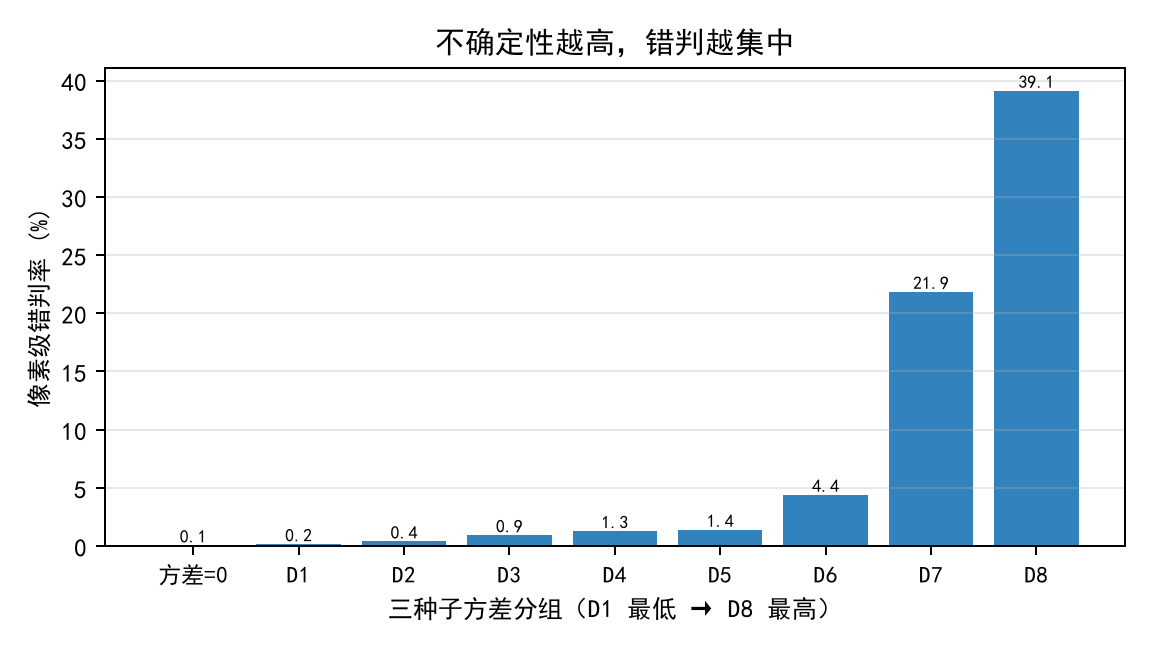
\includegraphics[width=0.72\textwidth]{../outputs/figures/q1_uncertainty.png}
\caption{按三种子方差分组的像素级错判率（最左为方差为零的像元）}
\label{fig:q1-unc}
\end{figure}

方差最大的十分位组只占测试像元的 $6.7\%$，却贡献了 \textbf{55.6\%} 的错判。这为问题三提供了直接可用的筛选规则：在「高方差区」宜以保守策略（按淹没处理）配置救援资源，在「零方差区」可信任模型结论以节省复核成本。不确定性因此不是副产品，而是问题二、三之间的信息通道。

\subsubsection{块级栅格产品与契约校验}

为验证四件套在生产意义上的可用性，选取测试集中瓦片最完整的子块（$4\times4=16$ 个瓦片，$1024\times1024$ 像元）按原始 EPSG:4326 网格直接拼接，输出概率、掩膜、不确定性三张单波段栅格与元数据（图 \ref{fig:q1-block}）。拼接不做重采样，左上角由块内西北角瓦片中心反推，因此几何上与附件严格对齐。

\begin{figure}[H]
\centering
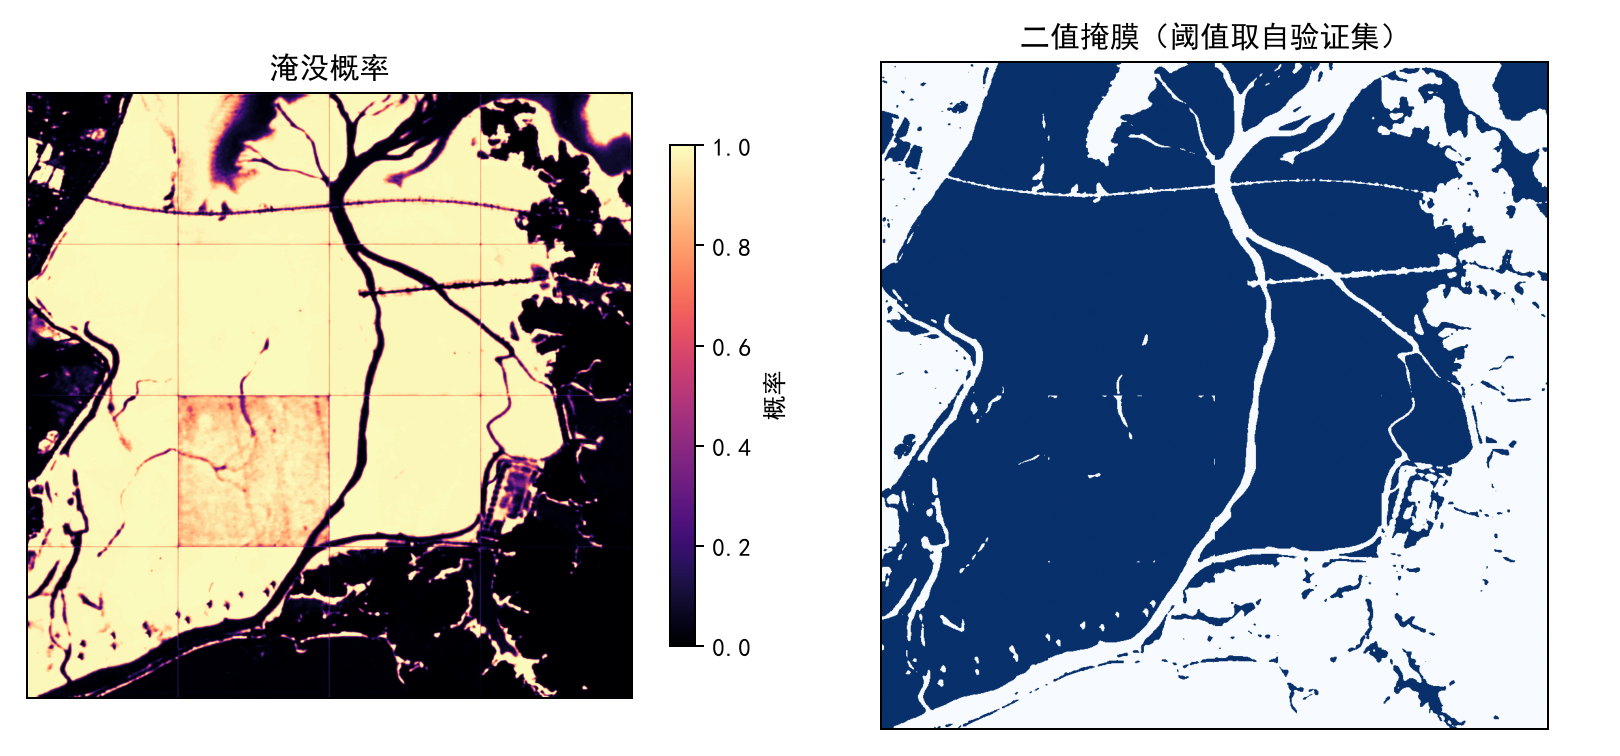
\includegraphics[width=0.95\textwidth]{../outputs/figures/q1_test_block.png}
\caption{测试块的四件套栅格产品：淹没概率（左）与二值掩膜（右）}
\label{fig:q1-block}
\end{figure}

该块真值淹没 638\,842 像元（$48.059\ \mathrm{km^2}$），预测 645\,789 像元（$48.582\ \mathrm{km^2}$），\textbf{预测/真值 $=1.011$}，块级面积误差仅 $1.1\%$——明显优于切片累计的 $+9.3\%$，说明误差在块间相互抵消，\emph{区域总量}比\emph{单块总量}更可靠。用合同校验脚本检查，四件套的坐标系、变换、宽高、单波段约束全部通过，仅有「交付栅格为 EPSG:4326 而非分析用 EPSG:32649」一条警告，属预期（合同要求保留附件原生网格）。

\subsection{误差来源与局限}
\label{sec:q1-limit}

\begin{enumerate}
\item \textbf{缺少显式的时序对比。} 本文把灾前光学作为辅助通道送入网络，但未构造「灾前水体掩膜—灾后 SAR」的显式变化特征。由于标签语义已核验为新增淹没，网络必须自行从 5 通道中学到「灾前这里是不是水」，这是西片区误报偏高的可能原因之一。
\item \textbf{瓦片独立推理。} 当前按 $256\times256$ 瓦片独立推理，块内可见轻微接边痕迹（图 \ref{fig:q1-block} 中部的水平纹理突变即瓦片边界）。重叠推理 + Hann 窗融合可消除该现象，但由于块级面积误差仅 $1.1\%$，本文判断其对结论影响有限，列为后续改进。
\item \textbf{区域覆盖不完整。} 交付的栅格产品目前只覆盖一个测试块，用于验证契约与出图流程；全区域的概率拼接与总淹没面积需要按同一流程批处理，属工程量而非方法问题。
\item \textbf{阈值与面积的可迁移性。} 表 \ref{tab:q1-thr} 的负结果说明，任何依赖单一阈值把面积「校平」的做法在跨区应用时都不可靠。实际使用时应以概率与不确定性为主，面积为区间估计。
\end{enumerate}

\subsection{小结与对后续问题的接口}
\label{sec:q1-summary}

问题一的主要工作与结论可归纳为：

\begin{enumerate}
\item 用椭球面积口径（中位 $74.94\ \mathrm{m^2}$/像元）替代 $100\ \mathrm{m^2}$ 的习惯口径，避免 $33\%$ 的系统性高估；
\item 标签语义经灾前亮度、暗水体占比与 SAR 强度比值三重证据定稿为 \mbox{\texttt{newly\_inundated\_only}}，即在合同中禁止再做灾前水体差集；
\item 查明附件为 5 片镶嵌而非 90 个独立块，据此建立 90 个子块的分层划分（692/151/157，水体占比 $0.196/0.144/0.209$，块中心最近距 $5.705\ \mathrm{km}$）；
\item 以 U-Net 三种子集成取得测试集 \textbf{IoU $0.8057$、F1 $0.8924$、召回率 $0.934$}，较随机森林基线提升 9.7 个 IoU 点；
\item 概率经保序回归校准（ECE $0.0161$），阈值在验证集冻结为 $\tau=0.46$；
\item 三种子方差与错判率同向（最高分组错判率 $39.1\%$，最低 $0.17\%$），可作为问题三的复核优先级信号。
\end{enumerate}

对后续问题的接口有三条约定：其一，交给问题二、三的概率栅格为 float32、NoData $=-9999$，掩膜为 uint8、忽略值 $255$，四件套同名同网格；其二，$\tau=0.46$ 是交付阈值，其他问题可在同一概率图上自行扫描阈值做敏感性分析，但\textbf{不得}重新训练或修改掩膜；其三，面积一律按椭球像元面积换算，并以 $\pm10\%$ 的区间报告，不承诺像元级面积精度。